\documentclass{article}
\usepackage{hyperref}
\usepackage{enumitem}
\usepackage[margin=1in]{geometry}
\usepackage{graphicx}
\usepackage{fancyhdr}
\usepackage{minted}
\usepackage{float}
\graphicspath{{Images/}}

\hypersetup{
	colorlinks=true, %set true if you want colored links
	linkcolor=black,  %choose some color if you want links to stand out
}

\pagestyle{fancy}
\rfoot{
\includegraphics[scale=0.4]{IITlogo}}

\title{ECE 100 Laboratory 05 Instructions }
\author{Illinois Institute of Technology ECE Department}
\date{Last Modified: \today}



\begin{document}
	\maketitle
	
	\paragraph{Lab Objective} Build an obstacle avoiding robot to compete in Competition 2. The most optimal robot will complete the course in its entirety in the shortest amount of time. 
	
	
\section{Hardware Installation}
	\paragraph{} Below are the instructions on how to properly assemble the obstacle avoidance robot. Please follow the instructions as listed to complete the build by the end of the Lab section. The instructions provided below are adapted from the OSOYOO provided instructions for your ease of use. If you wish to have additional support in the build process, navigate to the following link for a video tutorial. 
\vspace{1em}
 
	\href{https://osoyoo.com/2020/05/12/osoyoo-v2-1-robot-car-kit-lesson-4-tracking-line-robot-car/}{Video Tutorial Link}
\vspace{1em}

\textbf{Before you begin: Please note that you can make any changes to your robot that you see fit. You are welcome to add additional sensors, remove components, and outfit your robot as you see fit. Components from your teammates’ kits can be used for this purpose as well.}

\begin{enumerate}
	\item Start the installation from the previous status of lab 1. Remove the wiring connections from the IR sensor (if applicable). It is not necessary to remove the sensor entirely. 
	
	\item Install servo motor at the front of upper car chassis with 2pcs M2.2*8 self-tapping screws. Make sure that the output shaft of the servo is mounted inwards towards the car, the opposite of what is shown in the image below. The white rotating shaft should be closest to the OSOYOO logo.
	
	\begin{figure}[H]
		\centering
		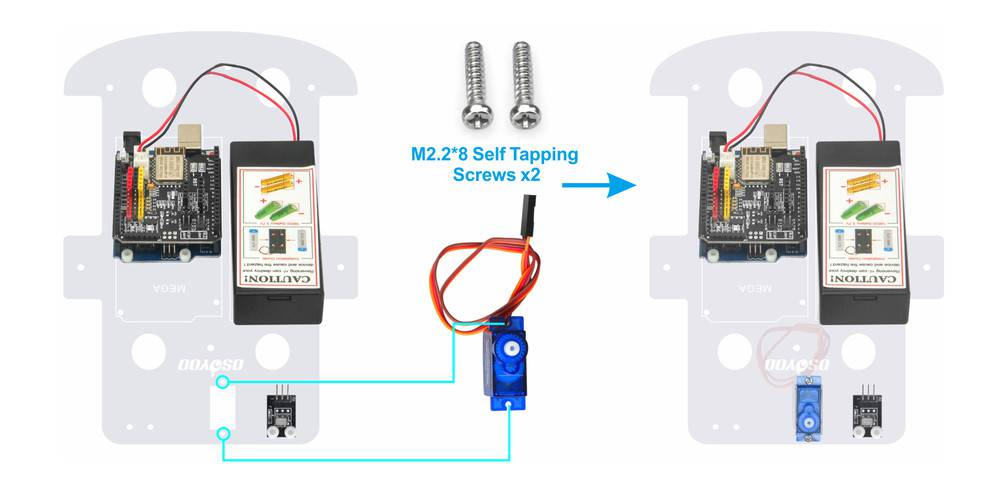
\includegraphics[width=0.7\linewidth]{Images/image2}
		\label{fig:image2}
	\end{figure}

	\item Install the Ultrasonic Module to mount holder with 4 M1.4*8 screws and M1.4 nuts. 
	
	\begin{figure}[H]
		\centering
		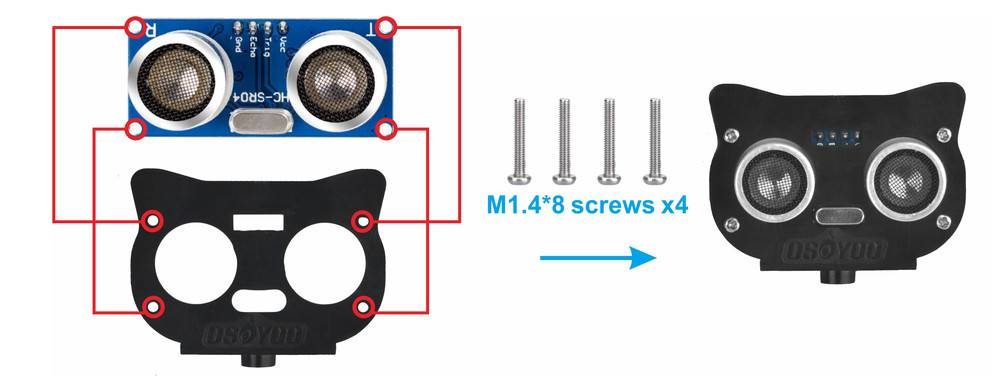
\includegraphics[width=0.7\linewidth]{Images/image3}
		\label{fig:image3}
	\end{figure}
	
	\item Install mount holder for Ultrasonic Module on servo motor with M2*4 Self Tapping screw.
	
	\begin{figure}[H]
		\centering
		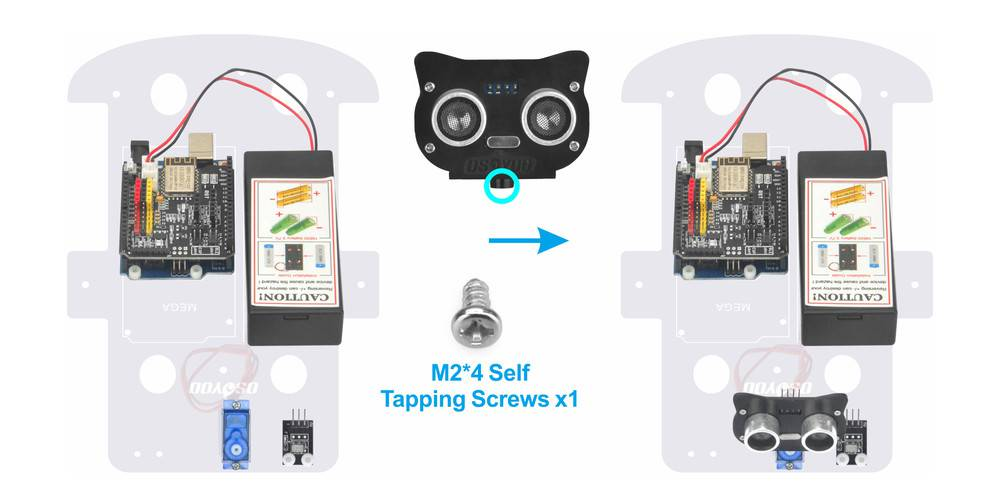
\includegraphics[width=0.7\linewidth]{Images/image4}
		\label{fig:image4}
	\end{figure}
	
	\item  Install Buzzer module at the back of upper chassis as sown in the image below. The pins for jumper cables should be facing inwards on the chassis. Use 1 pc M3 plastic screw, M3 plastic pillar, and M3 plastic nut to install.
	
	\begin{figure}[H]
		\centering
		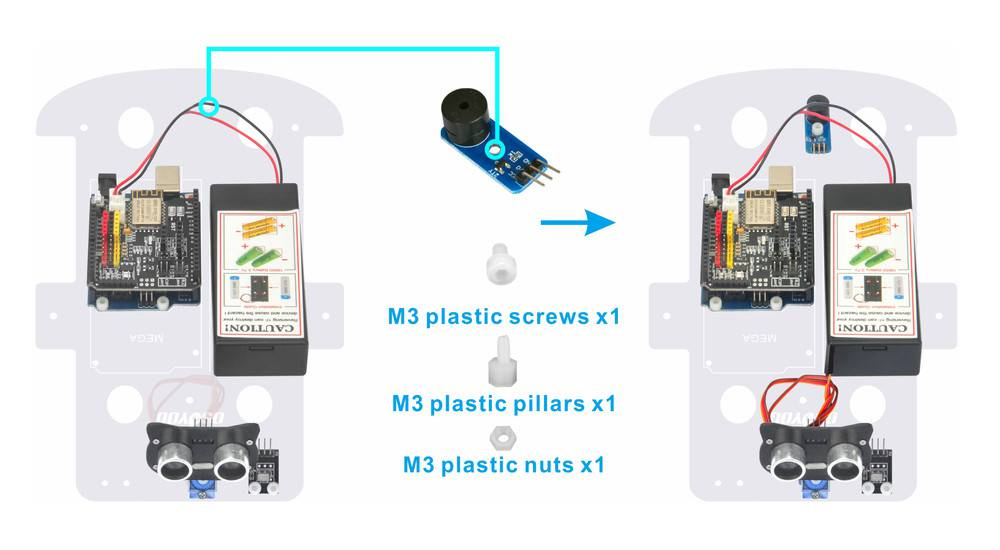
\includegraphics[width=0.7\linewidth]{Images/image5}
		\caption{}
		\label{fig:image5}
	\end{figure}
	
	\item Wire the SG60 servo motor to the motor driver and WiFi shield as shown in the image below. In order to access the motor driver, it is necessary to remove the upper level of the chassis. To do this, unscrew the top screw on each of the pillars. This will be enough to have access to the motor driver. Wire the motor driver and WiFi shield completely before replacing the top level of the chassis.
	
	\begin{figure}[H]
		\centering
		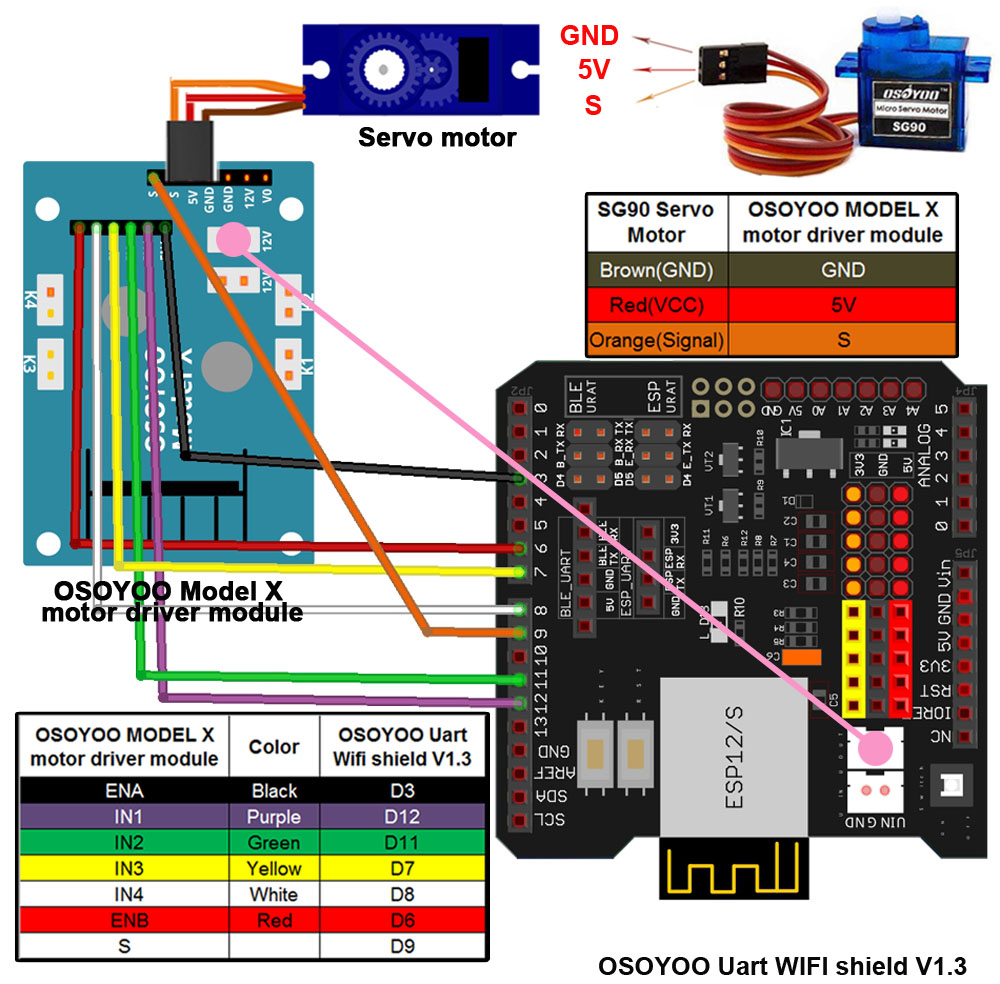
\includegraphics[width=0.7\linewidth]{Images/image6}
		\label{fig:image6}
	\end{figure}
	
	\item Connect the ultrasonic module and buzzer with the WiFi shield as shown in the connection diagrams below. 
	
	\begin{figure}[H]
		\centering
		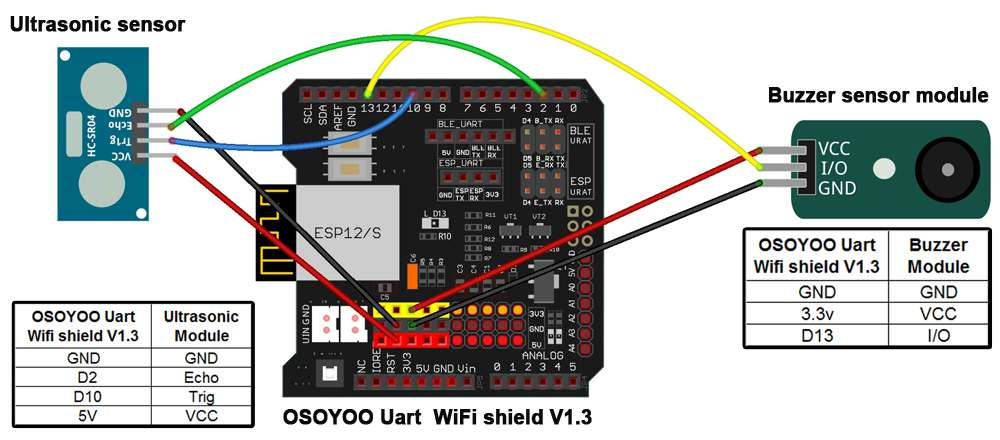
\includegraphics[width=0.7\linewidth]{Images/image7}
		\label{fig:image7}
	\end{figure}
	
\end{enumerate}

\textbf{Hardware installation is complete!}


\section{Software Installation}
\begin{enumerate}
	\item Ultrasonic Sensor Calibration: {\color{red}\textbf{(IMPORTANT)}}
	\begin{enumerate}[label=\alph*.]
		\item Download \href{https://osoyoo.com/driver/arduino_servo_car/servo.zip}{this file}
		
		\item Unzip the above file and run the servo.ino file in your car.
		
		\item Your servo will move from left to right and finally stop to center position. If your ultrasonic sensor is not facing to front direction. Please release your ultrasonic sensor from the servo head, reposition its direction to the front, then fasten the sensor screw to fix its direction.  See video from 7:40 to 8:10.
		
		\item After you have changed the sensor direction, please run v2smartcar-lesson5.ino sketch again. Your car will begin to do obstacle avoidance driving.
	\end{enumerate}
	
	\item Choose the corresponding board/port for your project, upload the provided sketch to the board.
	
	\item After turning on the battery, you will hear a long beep sound, then the servo will make some movement and finally stops in a direction for 5 seconds.
	
	\item During these first 5 seconds, you must make sure the Ultrasonic sensor(two eyes) is facing straight forward.
	\begin{enumerate}[label=\alph*.]
		\item If it is not facing straight forward, you should turn off the battery immediately and remove the sensor from the servo, reinstall it and make it facing straight forward as in the following picture. Otherwise, the obstacle avoidance program will not work properly.
		
		\begin{figure}[H]
			\centering
			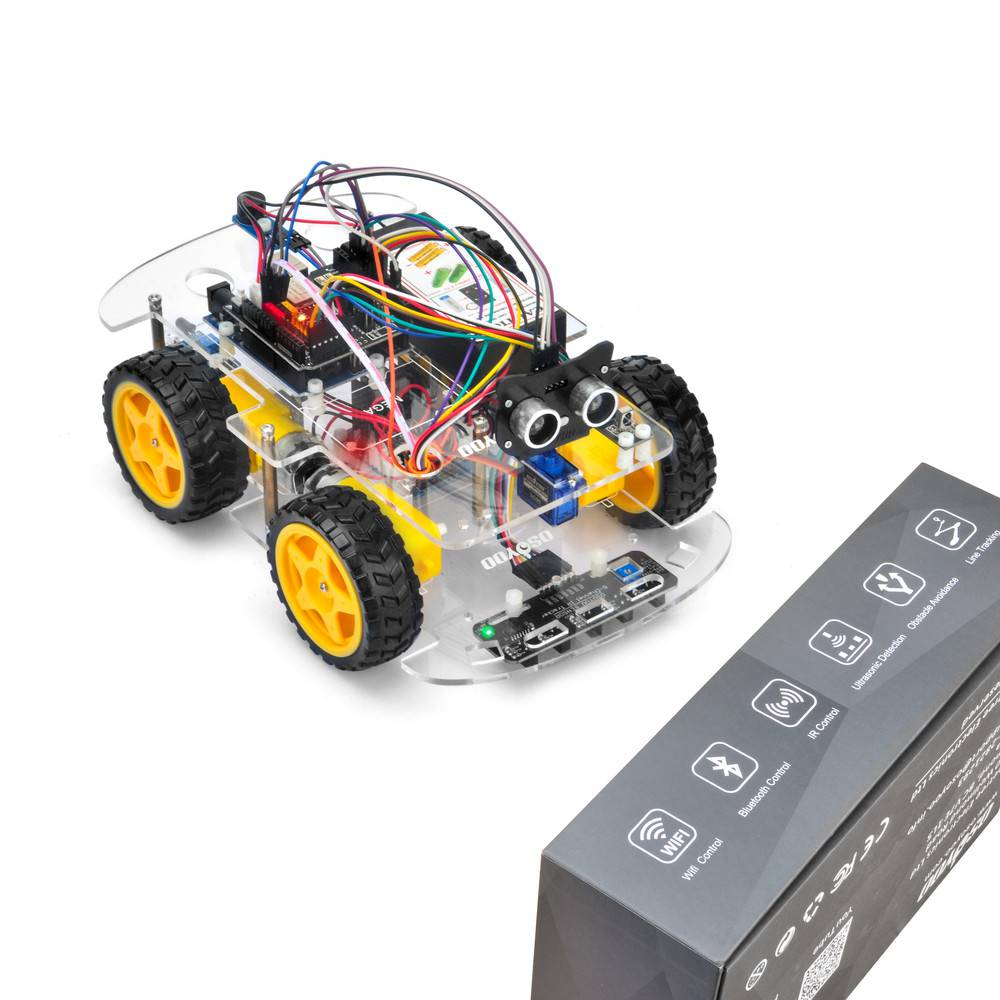
\includegraphics[width=0.5\linewidth]{Images/s4}
			\label{fig:s4}
		\end{figure}
		
		\item After adjusting the sensor direction, turn on the battery again. After hearing the long beep, the sensor should face the front straight forward. If its direction is not, turn off the battery and do direction alignment again.
	\end{enumerate}

	\item Run the sample code provided. Now be creative and come up with your own solution.
	

\end{enumerate}

\end{document}